
\section{Calorimetry}\label{sec:energyreco}
\subsection{Scope of the energy reconstruction}
In this analysis we restrict ourselves to the measurement of the deposited energy in the TPC of the visible particles in the final state of the $\nu_e$ CC0$\pi$-Np neutrino interaction. Our signal has in its final state, by definition, one electron and at least one proton, with no other visible particles. The energy of the electron is measured by converting the reconstructed charge of all the shower-like objects into deposited energy, as described in Section \ref{sec:showerenergy}. The energy of the protons, instead, can be measured by converting the track length of the reconstructed tracks into deposited energy, using the tabulated stopping power of protons in the liquid argon, with the procedure described in \ref{sec:protonenergy}. The total reconstructed energy corresponds to the sum of the reconstructed energies, corrected by the calibration factors calculated below, and is referred to as $E_{\mathrm{corr}}$. This quantity is then compared with the total kinetic energy of the particles above detection thresholds and corrected by a calibration factor to obtain an estimate of the deposited energy $E_{\mathrm{deposited}}$ (Section \ref{sec:deposited}).


\subsection{Electron energy reconstruction and calibration}\label{sec:showerenergy}
The reconstructed energy $E_{\mathrm{reco}}^{e}$ of a shower-like object is measured converting the charge of the associated hits into deposited energy in the TPC. It is calculated by multiplying the reconstructed charge ($e^{-}_{\mathrm{reco}}$) from hits associated with the reconstructed shower by the calibration factor \cite{Acciarri:2017sjy}:
\begin{equation}
\frac{E_{\mathrm{reco}}^{e} \mathrm{(MeV)}}{e^{-}_{\mathrm{reco}}} = 1.01\frac{e^-}{e^{-}_{\mathrm{reco}}} \times \frac{23.6~\mathrm{eV}}{e^-} \times 10^{-6} \frac{\mathrm{MeV}}{\mathrm{eV}} \times \frac{1}{R} = 3.85\times10^{-5},\label{eq:calib}
\end{equation}
where:
\begin{itemize}

\item the correction factor $1.01\frac{e^-}{e^{-}_{\mathrm{reco}}}$ is obtained measuring the true number of collected electrons $e^{-}$ on the wires using a sample of stopping muons, fitting the $dE/dx$ vs. residual range to values for argon as tabulated by the PDG \cite{PhysRevD.98.030001};
\item $\frac{23.6~\mathrm{eV}}{e^-}$ is the work function for ionizing an argon atom \cite{Shibamura:1975zz};
\item $R = 0.62$ is the recombination factor obtained with the Modified Box Model \cite{Acciarri:2013met} at MicroBooNE's electric field of 270~V/cm.
\end{itemize}

The reconstructed energy is obtained summing the energy of each hit from the reconstructed showers produced by a simulated electron in the collection plane, produced by a $\nu_{e}$ CC0$\pi$-Np interaction. The starting point of the simulated electron and the starting point of the reconstructed showers are required to be within the fiducial volume. 
Figure \ref{fig:ecalib} shows the calibration slope necessary to convert the electron reconstructed energy $E_{\mathrm{reco}}^{e}$ into true electron energy $E^{e}$. The true energy spectrum has been divided in 10 bins of equal size in the 30-2030~MeV range. Since the reconstructed energy distributions in each true energy bin are asymmetric, the data points are obtained fitting the distributions with a GaussExp function \cite{Das:2016stf}, in order to estimate the most probable value (MPV). The GaussExp function consists of an exponential tail stitched to a Gaussian core and it is often use to measure lossy processes such as the energy reconstructed in a calorimeter. The coordinate on the $E^{e}$ axis are given by the mean of the true energy distribution for each bin. The vertical error bars correspond to the full width at half maximum (FWHM) of the fitted function. The true energy distribution and the reconstruction energy distribution for every bin are shown in Figure \ref{fig:e_spectra}.

\begin{figure}[htbp]
\centering
\begin{overpic}[width=0.95\linewidth]{figures/e_spectra.pdf}
\end{overpic}
% 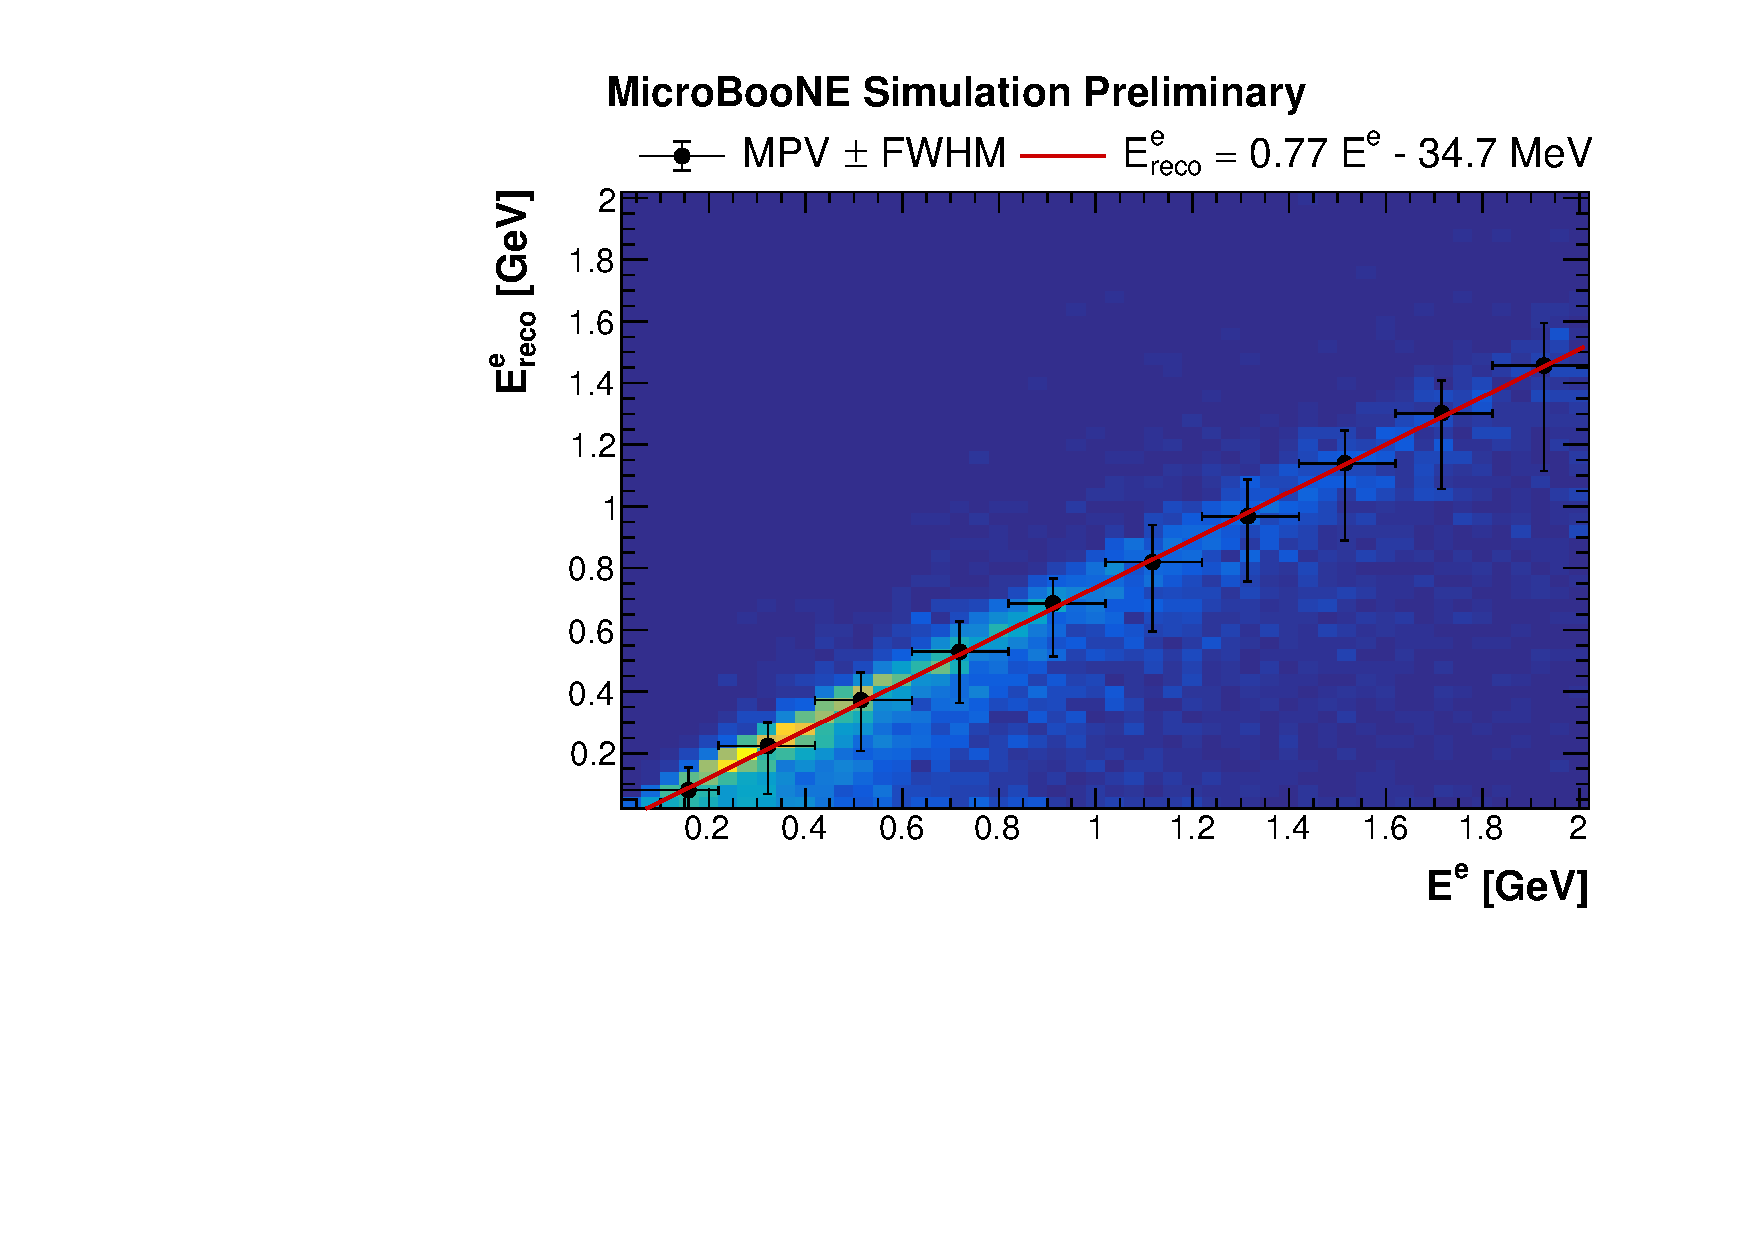
\includegraphics[width=0.65\columnwidth]{figures/ecalib.pdf}
\caption{Reconstructed and true energy distribution for 10 intervals of equal size in the 30-2030 MeV energy range. The reconstructed energy distribution have been fitted with a GaussExp function.}
\label{fig:e_spectra}
\end{figure}


The linear fit of the most probable value points, shown in Figure \ref{fig:ecalib} gives:
\begin{equation}
E_{\mathrm{reco}}^{e} = 0.77~E^{e} - 34.7~\mathrm{MeV}.
\end{equation}
The energy of the shower, corrected by the calibration factor is then defined as:
\begin{equation}
E_{\mathrm{corr}}^{e} = (E_{\mathrm{reco}}^{e} + 34.7~\mathrm{MeV})/0.77.
\end{equation}

\begin{figure}[htbp]
\centering
\begin{overpic}[width=0.7\linewidth]{figures/ecalib.pdf}
\end{overpic}
% 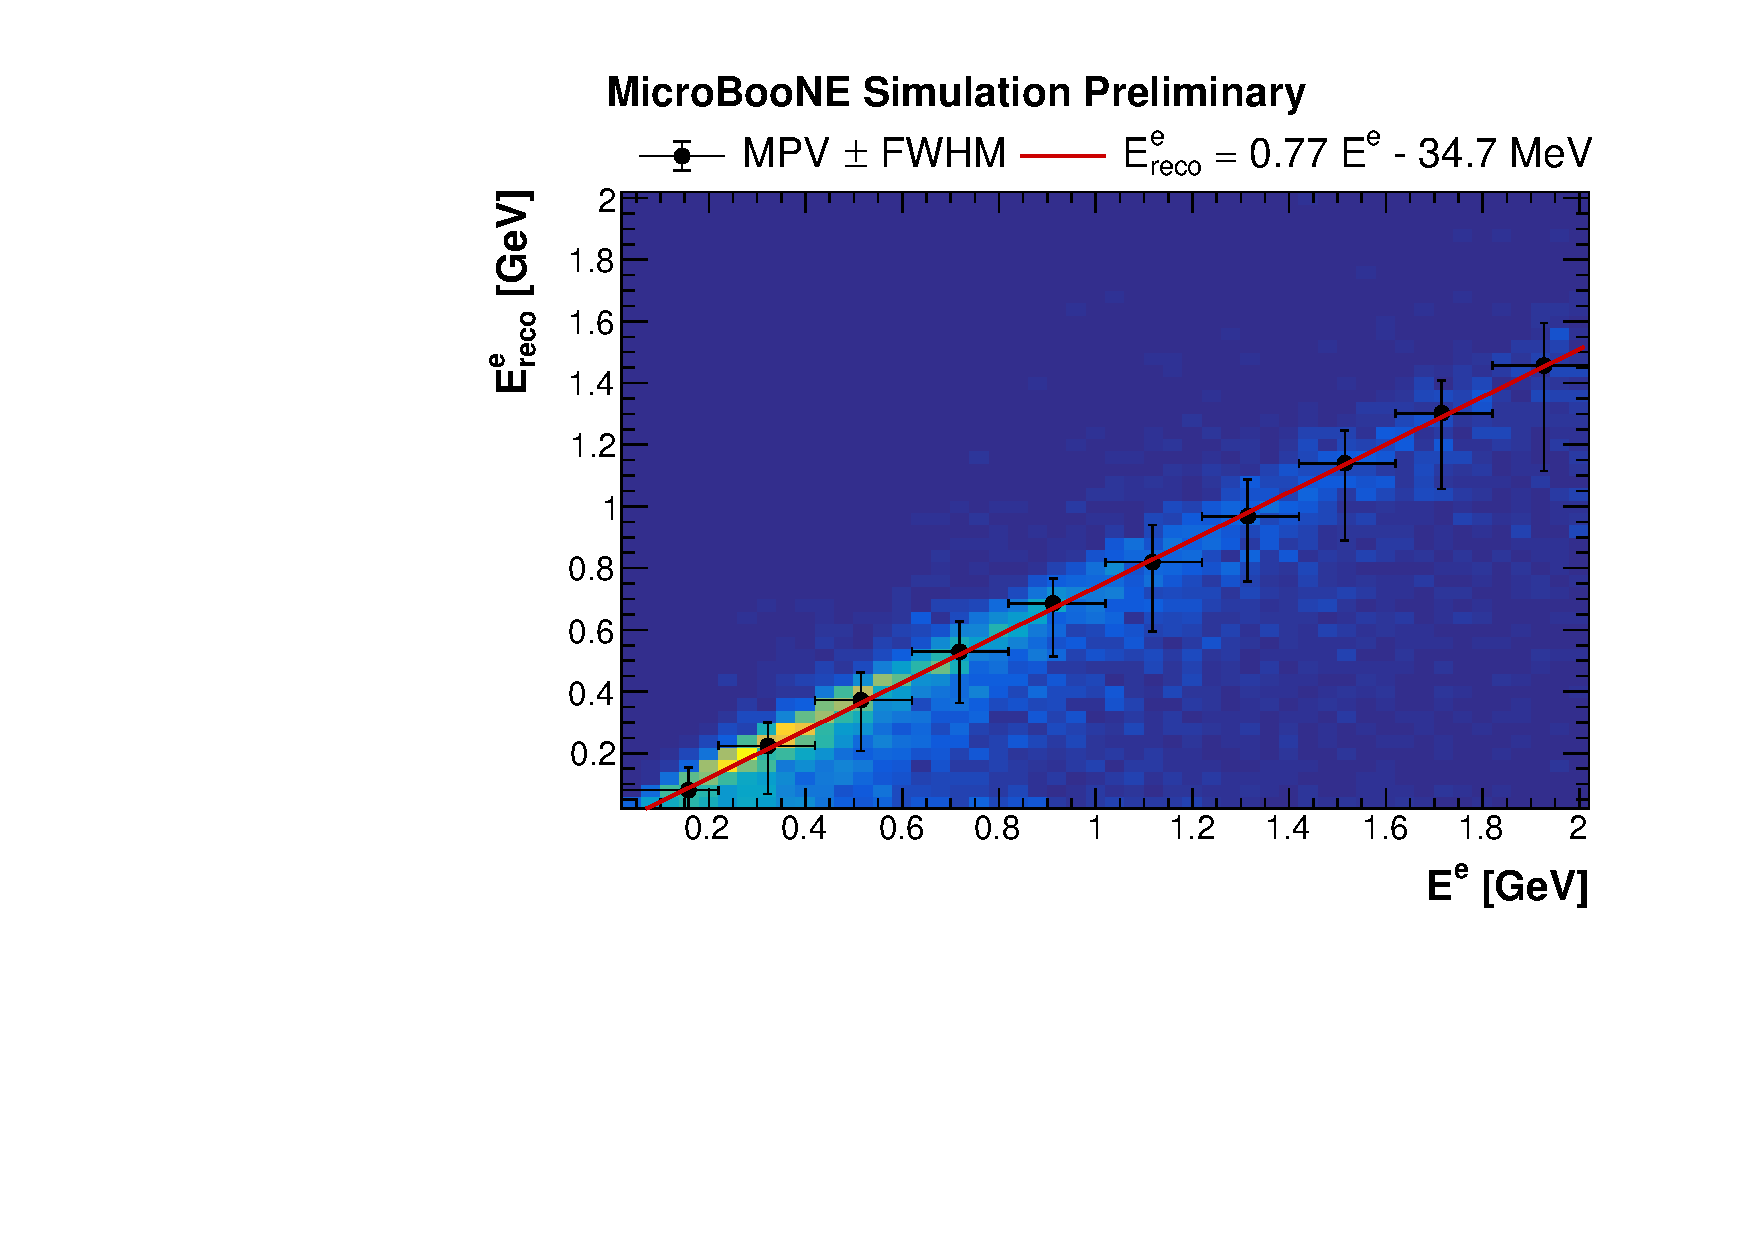
\includegraphics[width=0.65\columnwidth]{figures/ecalib.pdf}
\caption{Bi-dimensional histogram of true electron energy $E^{e}$ vs. reconstructed electron energy $E_{\mathrm{reco}}^{e}$. The reconstructed electron energy is measured summing the energy of each hit associated to reconstructed showers produced by the simulated electron. The black points are obtained measuring the most probable value of the $E_{\mathrm{reco}}^{e}$ distribution for each $E^{e}$ bin, measured by a GaussExp fit.}
\label{fig:ecalib}
\end{figure}

It is also possible to measure the energy resolution in the simulation by calculating the normalised difference $E_{\mathrm{frac}}$ between the corrected reconstructed energy $E^e_{\mathrm{corr}}$ and the true electron energy $E^e$:
\begin{equation}
    E_{\mathrm{frac}} = \frac{E^e_{\mathrm{corr}}-E^e}{E^e}.
\end{equation}
Figure \ref{fig:electron_res} shows the $E_{\mathrm{frac}}$ distribution for 10 intervals of equal size between 30 and 2030~MeV and the GaussExp fit for each distribution.

\begin{figure}[htbp]
\centering
\begin{overpic}[width=0.95\linewidth]{figures/electron_res.pdf}
\end{overpic}
% 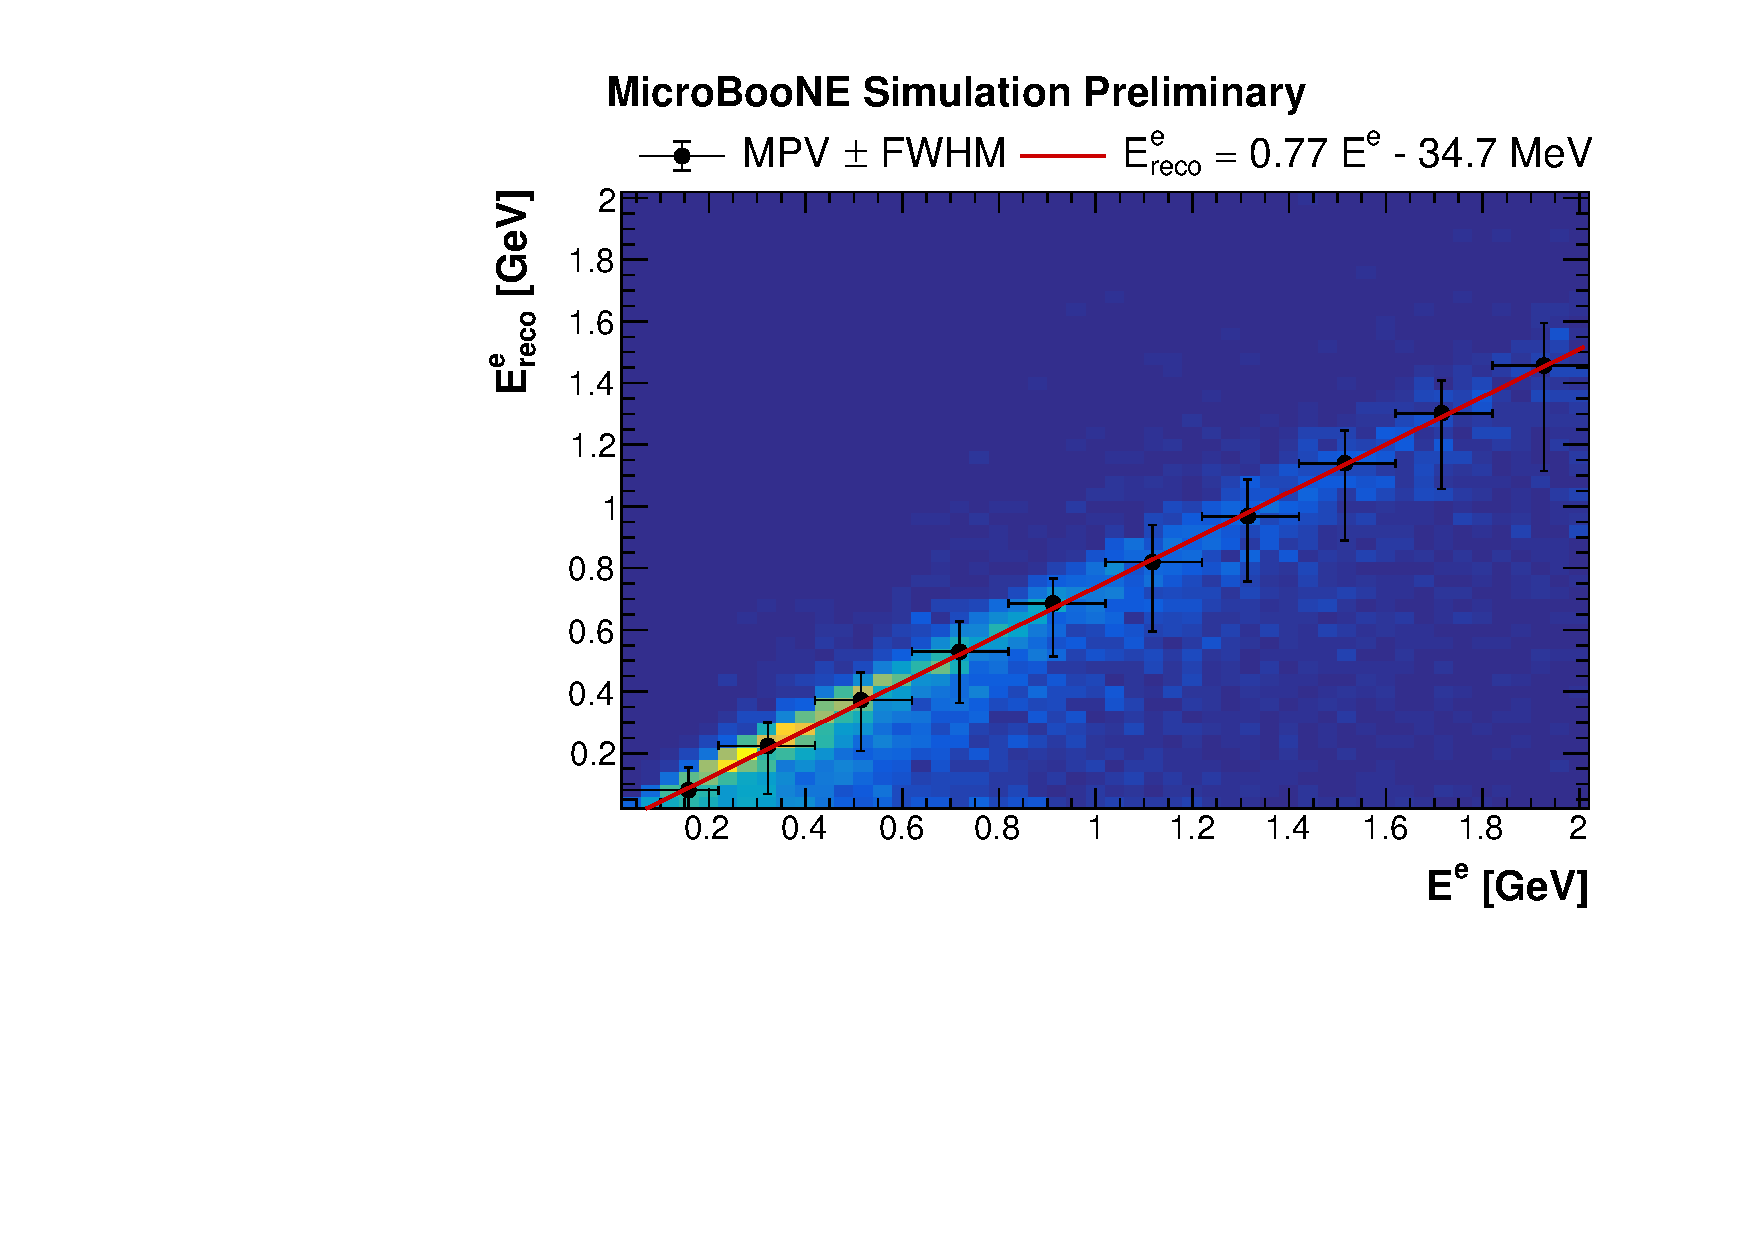
\includegraphics[width=0.65\columnwidth]{figures/ecalib.pdf}
\caption{Normalised energy difference $E_{\mathrm{frac}}$ for 10 intervals of equal size in the 30-2030 MeV energy range. The normalised energy difference distributions have been fitted with a GaussExp function (red line).}
\label{fig:electron_res}
\end{figure}

The fractional energy resolution can be defined as the ratio between the standard deviation of the Gaussian core $\sigma$ of the GaussExp function and the true electron energy $E_e$. Figure \ref{fig:sigma_e} shows the fractional energy resolution as a function of the true electron energy. The points can be fitted with the classic calorimeter resolution formula \cite{Fabjan:2003aq}:
\begin{equation}
    \frac{\sigma}{E} = \frac{a}{\sqrt{E}} \oplus \frac{b}{E} \oplus c,\label{eq:calo}
\end{equation}
where:
\begin{itemize}
    \item $a = 2.30\%$ is the stochastic term, which is caused by the intrinsic fluctuations of the development of the electromagnetic shower;
    \item $b = 7.53\%$ is the noise term, which comes from the electronics noise of the readout chain and represent the dominant contribution;
    \item $c = 1.21\%$ is the constant term, which is caused by detector non-uniformities (e.g. the presence of missing or unresponsive wires).
\end{itemize} 

\begin{figure}[htbp]
\centering
\begin{overpic}[width=0.85\linewidth]{figures/sigma_e.pdf}
\end{overpic}
\caption{Fractional energy resolution for 10 intervals of equal size in the 30-2030 MeV energy range. The points have been fitted the classic calorimeter energy resolution formula \eqref{eq:calo}.}
\label{fig:sigma_e}
\end{figure}


Another effect which contributes to the broadening of the energy resolution in MicroBooNE is caused by wrong or sub-optimal clustering: if the pattern recognition fails to group together all the hits that corresponds to the electromagnetic shower, or if it includes hits belonging to ionisation tracks (e.g. from cosmic muons), the reconstructed energy will be respectively smaller or larger than the true electron energy.
It is also important to underline that the energy resolution quoted here does not correspond to the intrinsic MicroBooNE energy resolution, but only to the energy resolution for the selected $\nu_e$ CC0$\pi$-Np events.

\subsection{Single proton energy reconstruction and calibration}\label{sec:protonenergy}
Proton energy reconstruction is obtained converting the reconstructed track length $L$ into deposited energy using the proton stopping power in liquid argon, as tabulated in \cite{pstar}. Liquid argon density $\rho_{\mathrm{LAr}}$ is assumed to be constant at 1.4~g/ml. Figure \ref{fig:proton} shows the proton kinetic energy as a function of the range of the proton in liquid argon (measured as $L \times \rho_{\mathrm{LAr}}$).

\begin{figure}[htbp]
\centering
  \begin{subfigure}{0.49\textwidth}
  \begin{overpic}[width=\linewidth]{figures/proton.pdf}
\put(120,640){\tiny{\textsf{\textbf{MicroBooNE Simulation Preliminary}}}}
\end{overpic}
%     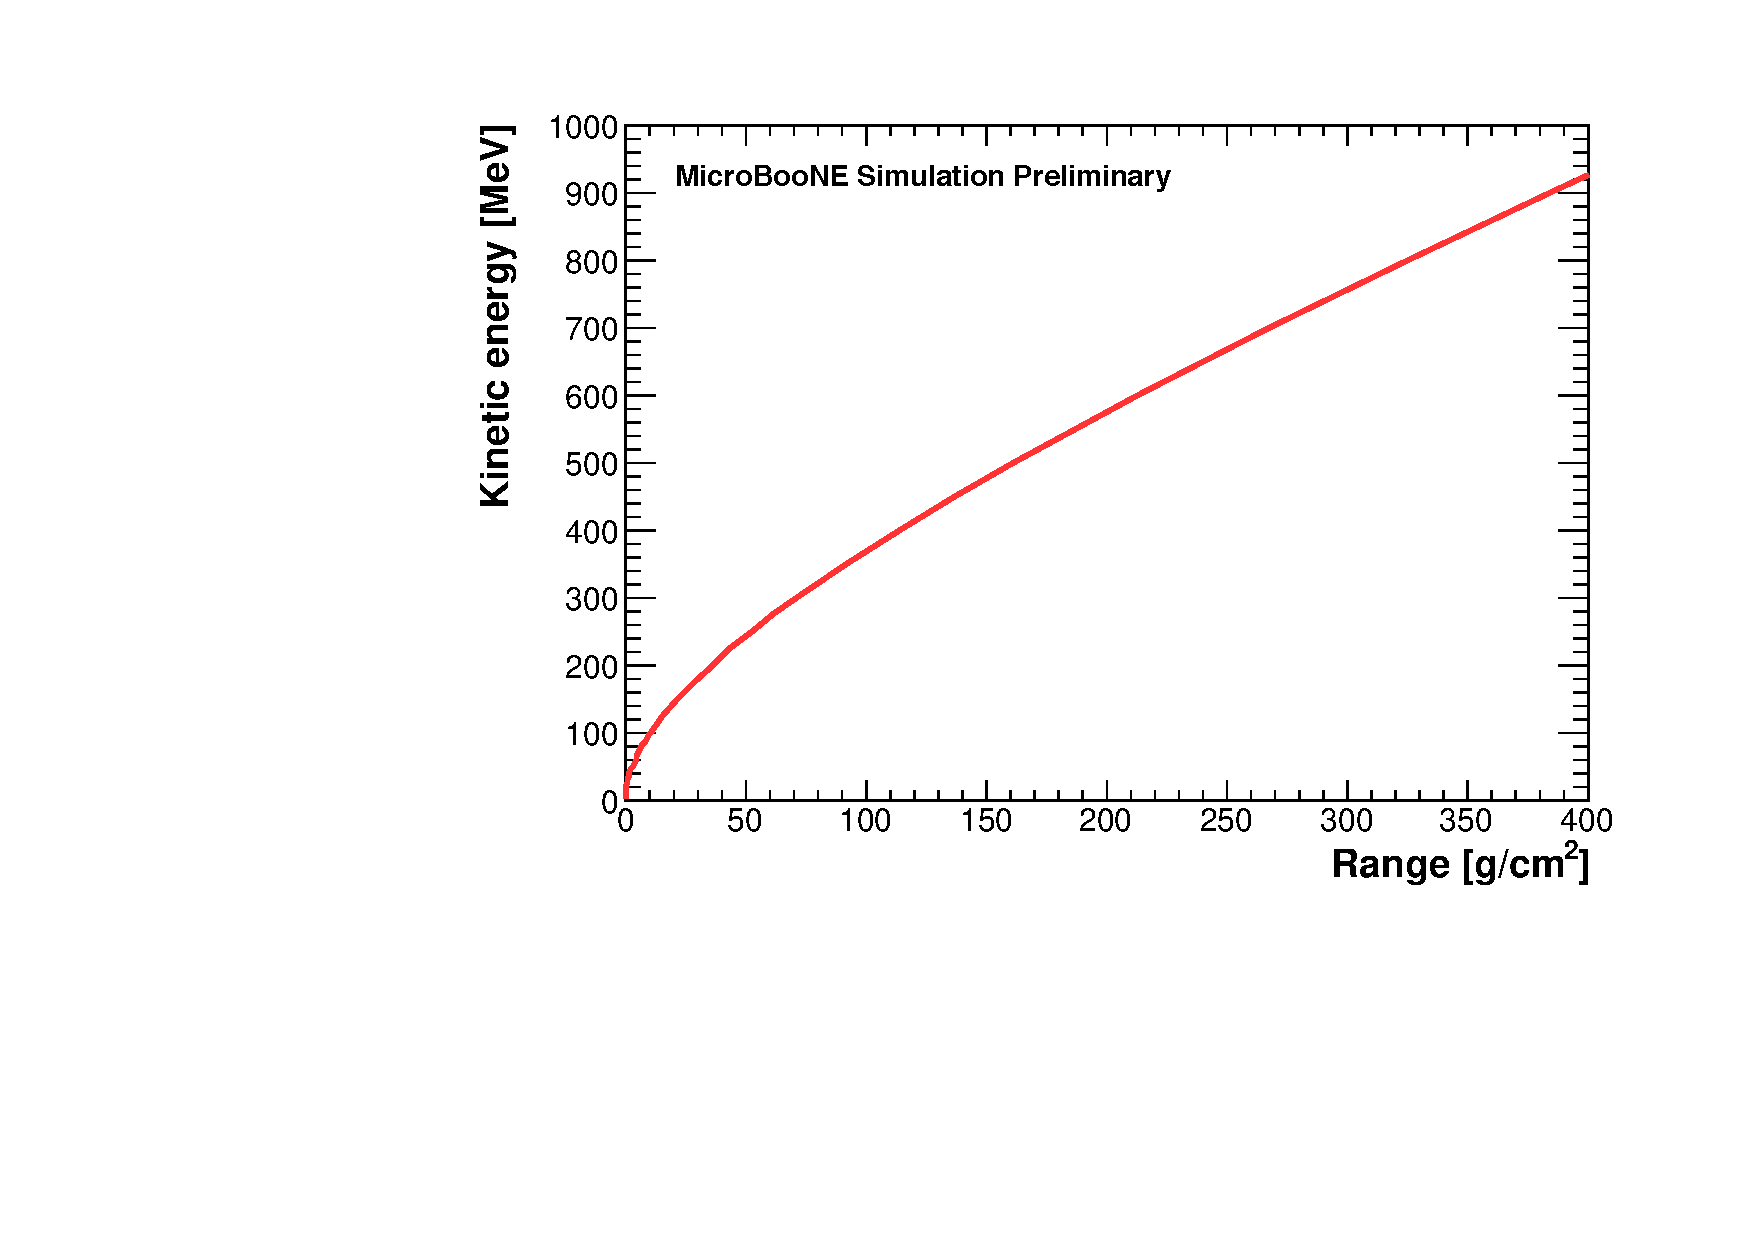
\includegraphics[width=\linewidth]{figures/proton.pdf}
    \caption{Proton kinetic energy as a function of the range of the proton in liquid argon.}\label{fig:proton}
  \end{subfigure}
  \begin{subfigure}{0.49\textwidth}
    \begin{overpic}[width=\linewidth]{figures/pcalib.pdf}\end{overpic}
% 	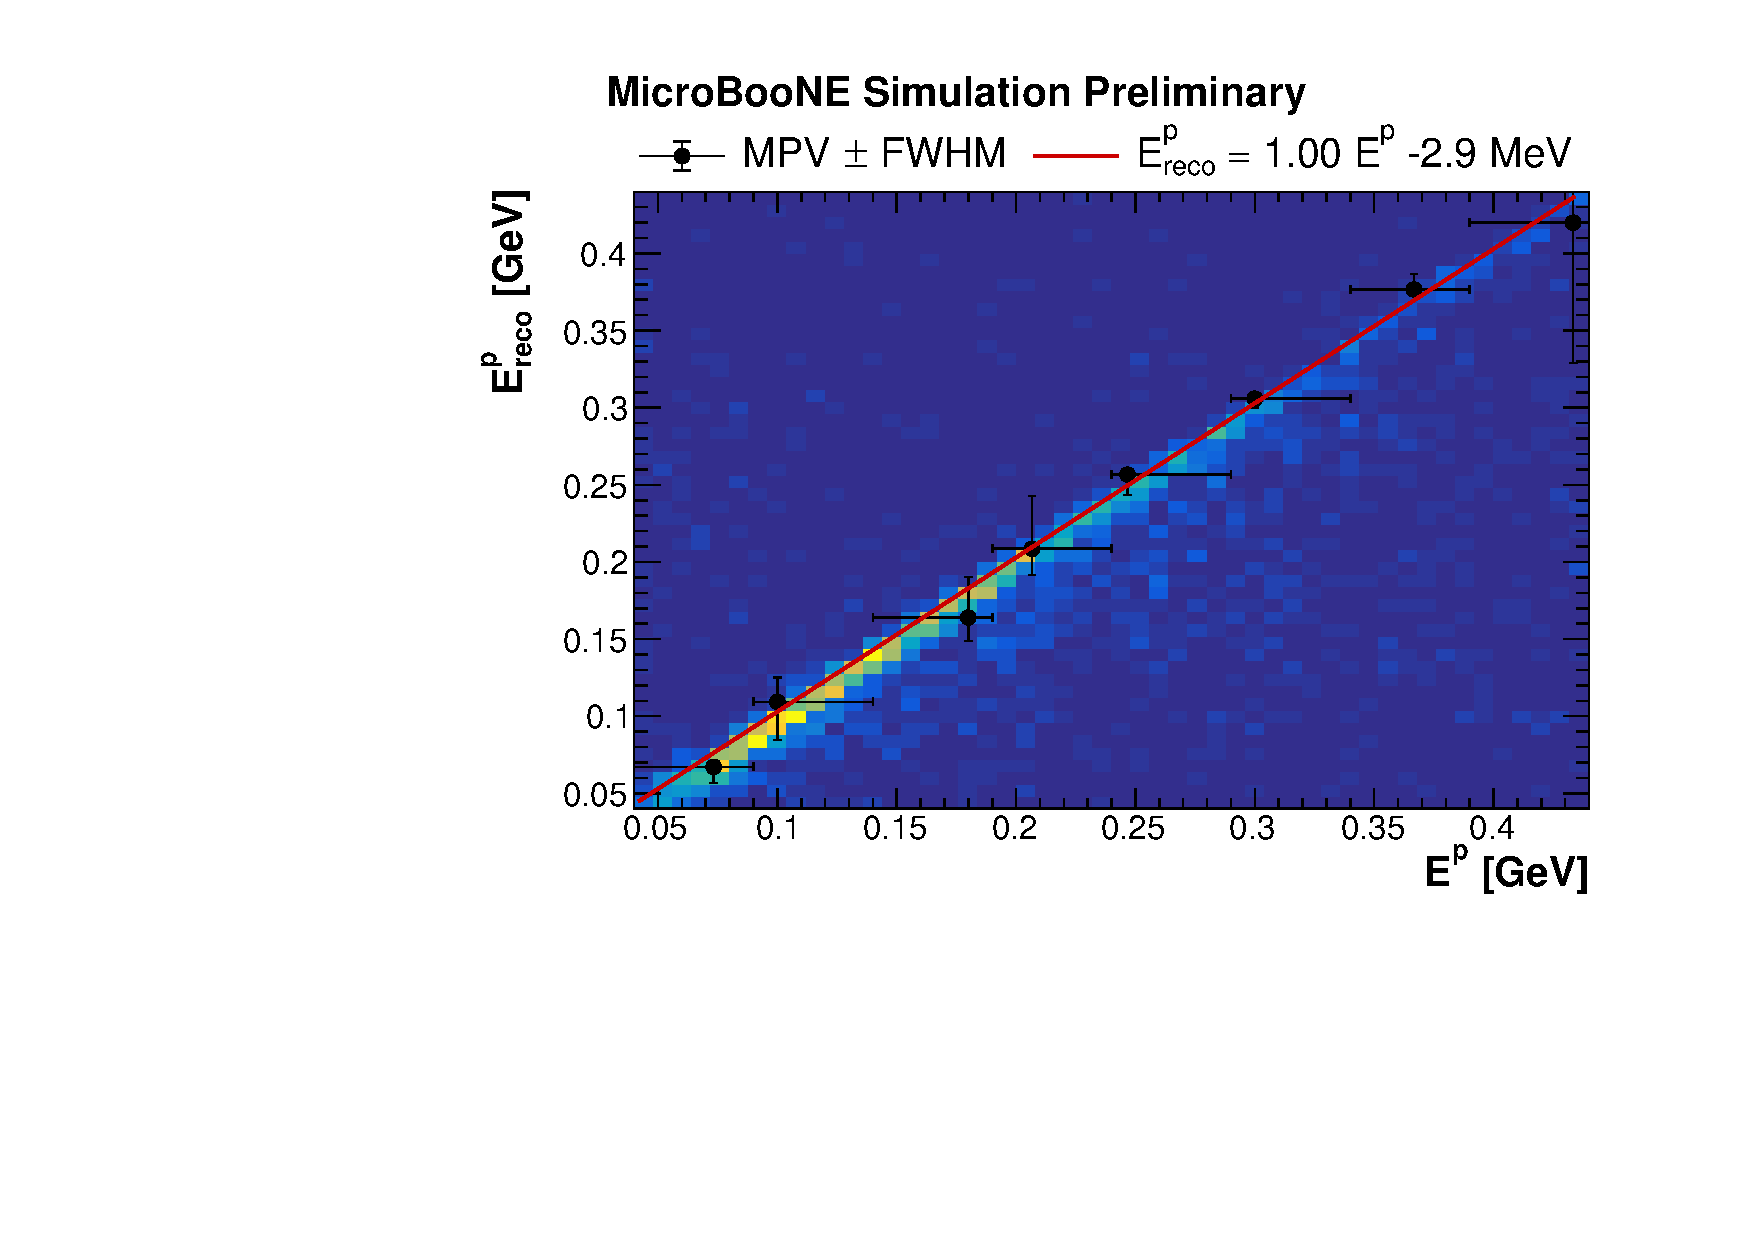
\includegraphics[width=\linewidth]{figures/pcalib.pdf}
     \caption{Bi-dimensional histogram of true proton energy $E^{p}$ vs. reconstructed proton energy $E_{\mathrm{reco}}^{p}$.}\label{fig:pcalib}
   \end{subfigure}
   \caption{The reconstructed proton energy is measured converting the reconstructed track length $L$ into deposited energy using the proton stopping power in liquid argon, as tabulated in \cite{pstar} (left). The calibration is calculated from a linear fit of the most probable values of the $E_{\mathrm{reco}}^{p}$ distribution for each $E^{p}$ bin (right).}
\end{figure}

The calibration constant has been obtained comparing the reconstructed energy of the proton with the true kinetic energy of the simulated proton, in a CC $\nu_{e}$ sample with only one proton in the final state. The true proton and the reconstructed tracks are required to be fully contained within the fiducial volume. Since protons are not minimum-ionising particles, in the case of two or more tracks (\emph{split tracks}) associated to the same proton, the reconstructed length of the tracks has been summed before calculating the corresponding kinetic energy.
Figure \ref{fig:pcalib} shows the calibration slope necessary to convert the proton reconstructed energy $E_{\mathrm{reco}}^{p}$ into true proton kinetic energy $E^{p}$. For each bin of the true proton energy, the most probable value of the corresponding proton reconstructed energy has been obtained with a GaussExp fit. A linear fit of the most probable values gives:
\begin{equation}
E_{\mathrm{reco}}^{p} = 1.00~E^{p} - 2.9~\mathrm{MeV}.
\end{equation}
The energy of the track, corrected by the calibration factor is then defined as:
\begin{equation}
E_{\mathrm{corr}}^{p} = (E_{\mathrm{reco}}^{p} + 2.9~\mathrm{MeV})/1.00
\end{equation}

\subsection{Deposited Energy Reconstruction}\label{sec:deposited}
It is possible to compare the total visible energy in the event $E_{\mathrm{k}}$, defined as the sum of the kinetic energies of the visible particles in the final state, with the sum of the reconstructed energies for shower-like ($E_{\mathrm{corr}}^{e}$) and track-like objects ($E_{\mathrm{corr}}^{p}$) for the selected $\nu_{e}$ CC0$\pi$-Np events. This quantity $E_{\mathrm{corr}}$ is defined as:
\begin{equation}
E_{\mathrm{corr}} = \sum^{N_{p}} E_{\mathrm{corr}}^{p} + \sum^{N_{e}} E_{\mathrm{corr}}^{e},
\end{equation}
where $N_{p}$ is the number of reconstructed tracks and $N_{e}$ is the number of reconstructed showers in the event. For events where we have two or more shower-like objects and no track-like objects, the shower-like object with the lowest proton $\chi^2$ score is chosen as proton candidate (see Section \ref{sec:proton_id}). In these cases we have $N_{p} = 1$ by definition.
The reconstructed energy does not include particles that do not interact in the liquid argon (such as neutrons) and charged particles with a kinetic energy below the detection threshold, defined in Section \ref{sec:eff}. Figure \ref{fig:nucalib} shows the calibration slope necessary to convert the the total reconstructed energy $E_{\mathrm{corr}}$ into visible energy $E_{\mathrm{k}}$. The plot has been obtained using the $\nu_{e}$ CC0$\pi$-Np + cosmic sample. A linear fit of the data points gives:
\begin{equation}
E_{\mathrm{k}} = 0.98~E_{\mathrm{corr}} - 28.5~\mathrm{MeV}.
\end{equation}
The reconstructed visible energy, corrected by the calibration factor is then defined as:
\begin{equation}
E_{\mathrm{deposited}} = (E_{\mathrm{corr}} + 28.5~\mathrm{MeV})/0.98
\end{equation}

Several effects can contribute to this calibration factor: among the others, the presence of regions with unresponsive of missing wires can cause an underestimation of the deposited energy. In the future, this effect can be limited by the use of the other two planes for calorimetric measurements.

\begin{figure}[htbp]
\centering
\begin{overpic}[width=0.85\linewidth]{figures/nucalib.pdf}
\end{overpic}\caption{Bi-dimensional histogram of total visible energy $E^{\mathrm{k}}$ vs. the total reconstructed energy $E_{\mathrm{corr}}$. Black points are obtained measuring the most probable value of the $E_{\mathrm{corr}}$ distribution for each $E_{\mathrm{k}}$ bin.} 
\label{fig:nucalib}
\end{figure}

In this analysis, we will use the quantity $E_{\mathrm{deposited}}$ as an estimate of the total visible energy in the event.

\subsection{Deposited energy binning}\label{sec:depositedenergy}
The binning of the deposited energy distribution must be carefully evaluated, since it is of fundamental importance in the calculation of the significance of an eventual excess. In this analysis, we require the events in a true $E_{\mathrm{k}}$ bin to fall in the same reconstructed $E_{\mathrm{deposited}}$ bin in at least 50\% of the cases for $\nu_e$~CC0$\pi$-Np events. A combination which satisfies this condition and maximises the number of bins in the $[0,3]$~GeV range is:
\begin{equation}
    E_{\mathrm{deposited}}\text{~bins} = [0, 0.2, 0.4, 0.6, 0.9, 1.25, 1.9, 3]~\text{GeV},
\end{equation}
which is then chosen as our binning for the $E_{\mathrm{deposited}}$ distributions.
Figure \ref{fig:migration} shows the migration matrix between $E_{\mathrm{deposited}}$ and $E_{\mathrm{k}}$. It shows the probability that an event with a true energy $E_{\mathrm{k}}$ in the $i$ bin has a reconstructed energy $E_{\mathrm{deposited}}$ in the same $i$ bin. Our binning criteria ensures that each element on the diagonal has a value larger than 0.50.

\begin{figure}[htbp]
\centering
\begin{overpic}[width=0.85\linewidth]{figures/migration.pdf}
\end{overpic}
\caption{Migration matrix between $E_{\mathrm{deposited}}$ and $E_{\mathrm{k}}$. It shows the probability that an event with a true energy $E_{\mathrm{k}}$ in the $i$ bin has a reconstructed energy $E_{\mathrm{deposited}}$ in the same $i$ bin.}
\label{fig:migration}
\end{figure}


\subsection{Measurement of the electromagnetic shower energy loss}\label{sec:dedx}
The mean energy loss per length of charged particles $\left\langle dE/dx\right\rangle$ can be described by the \emph{Bethe equation} as defined in Section 30.2.2 of \cite{PhysRevD.98.030001}:
\begin{equation}
    -\left\langle\frac{dE}{dx}\right\rangle = Kz^2\frac{Z}{A}\frac{1}{\beta^2}\left[\frac{1}{2}\ln\frac{2m_e c^2\beta^2\gamma^2 T_{\mathrm{max}}}{I^2}-\beta^2-\frac{\delta(\beta\gamma)}{2}\right],\label{eq:bethe}
\end{equation}
where $T_{\mathrm{max}}$ is the maximum possible energy transfer in a single collision, $I$ is the mean excitation energy, and $\delta(\beta\gamma)$ is a density correction. 

In material of moderate thickness such as LAr, the energy loss probability distribution is described by the asymmetric Landau distribution \cite{Landau:1944if}, which drives the mean of the energy loss of eq. \eqref{eq:bethe} into the tail of the distribution. For this reason, ``the
mean of the energy loss given by the Bethe equation [\dots] is thus ill-defined
experimentally and is not useful for describing energy loss by single particles'' (Section 30.2.7 of \cite{PhysRevD.98.030001}).
The most probable value of the Landau distribution, which should be used instead, is given by: 
\begin{equation}
    \Delta_p = \xi\left[\ln\frac{2mc^2\beta^2\gamma^2}{I}+\ln\frac{\xi}{I}+j-\beta^2-\delta(\beta\gamma)\right],\label{eq:landau}
\end{equation}
where $\xi = (K/2)\langle Z/A \rangle (x/b^2)$~MeV, $j=0.2$, and $x$ is the thickness of the material in $\mathrm{g}\cdot\mathrm{cm}^2$ (Section 30.2.7 of \cite{PhysRevD.98.030001}). 

An important feature of LArTPC technology is their ability to distinguish between electrons and photons in the final state by measuring their $dE/dx$. Photons that undergo pair-production, which is the dominant process above 10~MeV, produce a $e^+e^-$ pair. If the pair is boosted, the trajectories of the positron and the electron overlap, producing an average $dE/dx$ which is twice the one of a single, minimum-ionising electron. 

In MicroBooNE, the $dE/dx$ for electromagnetic showers is measured with a procedure analogous to the one developed by the ArgoNeuT collaboration and described in \cite{Acciarri:2016sli}. In this document, neutrinos were produced by the NuMI neutrino beam and the events were visually inspected to select electron and photon showers.

\begin{figure}[htbp]
\centering
\begin{overpic}[width=0.75\linewidth]{figures/evd_dedx.pdf}
\end{overpic}\caption{Event display of an electron shower candidate, showing the $1\times4$~cm area used for the $dE/dx$ calculation. Each small black rectangle corresponds to a reconstructed shower hit.}
\label{fig:evd_dedx}
\end{figure}

In our implementation, as a first step, all the hits of the collection plane within a rectangle of 4~cm along the direction of the shower and 1~cm perpendicular to the shower are collected, as shown in the event display in Figure \ref{fig:evd_dedx}.

Subsequently, the $dQ/dx$ for each hit is measured dividing the collected charge ($dQ$) by the pitch ($dx$) between each hit and the next one along the shower direction. The pitch corresponds to the distance in the TPC that a particle travels between its two projections  on adjacent wires, which is \emph{at least} the wire spacing (3~mm for MicroBooNE \cite{Acciarri:2016smi}). Electromagnetic showers aligned with the wire direction correspond to a large value of the pitch. 

The $dE/dx$ is calculated from the $dQ/dx$ using the calibration factor measured in Section \ref{sec:showerenergy}, eq. \eqref{eq:calib}.
Since the Landau distribution of the $dE/dx$ hit values has an asymmetric tail, we assign to the shower the median (and not the mean) of the $dE/dx$ hit distribution, as an estimation the most probable value. The median metric has been proved in \cite{Acciarri:2016sli} to be to most robust over a variety of box lengths.

\begin{figure}[htbp]
\centering
\begin{overpic}[width=0.75\linewidth]{figures/dedx.pdf}
\end{overpic}\caption{Area-normalised distributions for the measured $dE/dx$ for simulated electrons and photons.}
\label{fig:dedx_gamma_e}
\end{figure}

Figure \ref{fig:dedx_gamma_e} shows the area-normalised histograms of the $dE/dx$ in the collection plane for simulated electron and photon showers. The events below 1~MeV/cm correspond for both distributions to showers with a low number of associated hits, or where the shower was mostly aligned with the wires of the collection plane (having as such a high pitch value). Figure \ref{fig:pitch} shows the pitch distribution in the collection plane and a bi-dimensional histogram of the $dE/dx$ vs. the pitch for photon showers: events with a $dE/dx$ below 1~MeV/cm mostly correspond to a high value of the pitch. 

\begin{figure}[htbp]
  \begin{subfigure}{0.49\textwidth}
  \begin{overpic}[width=0.88\linewidth]{figures/pitch.pdf}
\end{overpic}
    \caption{Pitch distribution for simulated electron showers in the collection plane (log-scale).}
  \end{subfigure}\hfill
  \begin{subfigure}{0.49\textwidth}
    \begin{overpic}[width=\linewidth]{figures/dedx_vs_pitch.pdf}\end{overpic}
     \caption{Bi-dimensional histogram of measured $dE/dx$ vs. pitch for photon showers.}
   \end{subfigure}
   \caption{Electromagnetic showers aligned with the wire orientation will have a large pitch value and their measured $dE/dx$ will be shifted towards low values.}\label{fig:pitch}
\end{figure}

The electron showers have a peak around 2~MeV/cm, as expected. The photon showers, instead, have a peak around 4~MeV/cm and a second peak around 2~MeV/cm, which represent a limitation to our $e/\gamma$ separation capabilities. This peak is caused by mainly two effects:
\begin{itemize}
    \item photons that undergo Compton scattering will transfer most of their energy to the electron, producing a shower with the same $dE/dx$ of an electron. This effect decreases with the photon energy and is dominant below 10~MeV, as shown in Figure \ref{fig:compton};
    
    \begin{figure}[htbp]
    \centering
    \begin{overpic}[width=0.75\linewidth]{figures/compton.png}
    \end{overpic}\caption{Cross section of gammas on argon between 1 MeV and 1 GeV. Here, $\kappa$ refers to the pair production cross section for the nuclear field and electron field. Compton scattering is dominant below 10 MeV. From \cite{Acciarri:2016sli}.}
    \label{fig:compton}
    \end{figure}
    
    \item very asymmetric $\gamma\rightarrow e^+e^-$ pair production. When the positron and the electron do not overlap, the measured $dE/dx$ distribution will be peaked around 2~MeV/cm. The electron and the positron can also be produced with very different energies, as shown in Figure \ref{fig:asymmetry}. In this case, the distribution of the $dE/dx$ values in the $1\times4$ will have a mean value close to 2~MeV/cm. 
    
    \begin{figure}[htbp]
    \centering
    \begin{overpic}[width=0.75\linewidth]{figures/asymmetry.pdf}
    \end{overpic}\caption{Pair production relative cross-section as a function of the fraction of the photon energy $k$ transferred to either the electron or positron with energy $\epsilon$. From \cite{Caratelli:2018nob}.}
    \label{fig:asymmetry}
    \end{figure}
\end{itemize}

A comparison between the data and Monte Carlo distributions of the reconstructed showers $dE/dx$ is shown in Figure \ref{fig:dedx_datamc} of Section \ref{sec:bkg}.

\subsection{Particle identification of reconstructed tracks}\label{sec:proton_id}
The measurement of the $dE/dx$ along the reconstructed tracks allows to perform powerful particle identification, as demonstrated by a the ArgoNeuT collaboration in \cite{Acciarri:2013met}. 

This capability is particularly important for the search of low-energy electron neutrinos. A $\nu_e$ CC0$\pi$-1p neutrino interaction is topologically identical to a cosmic muon stopping in the LAr, since they both appear as a track with a small shower attached. However, the energy loss of a proton produced in a neutrino interaction is sensibly different from the one of a cosmic muon, for two main reasons:
\begin{itemize}
    \item the Bragg peak of the stopping cosmic muon corresponds to starting point of the Michel electron shower, while the Bragg peak of the proton track is far from the interaction vertex;
    \item the proton $dE/dx$ profile for protons differs from the $dE/dx$ profile for muons.
\end{itemize}
Being able to distinguish between proton and muon tracks is therefore essential in order to reject cosmogenic background. Events with a $\nu_{\mu}$ interaction with only a stopping muon in the final state can also be rejected with the same technique.

It is possible to parametrise the relation between the theoretical $dE/dx$ of a ionisation track and its \emph{residual range} with a power-law function:
\begin{equation}
    \frac{dE}{dx} = A R^b,
\end{equation}
where $A$, which has dimensions MeV/cm$^{1-b}$, and $b$, which is dimensionless, depend on the particle which produced the ionisation trail. The residual range $R$, in this case measured in centimetres, is the distance between a point on the track and its end ($R=0$ correspond to the track end-point).
Figure \ref{fig:range} shows the $dE/dx$ as a function of the residual range $R$ for several particle types. The values of $A$ and $b$ for each particle type are reported in Table \ref{tab:range}.

\begin{table}[htbp]
   \centering
   \caption{Stopping power parametrisation for various particle types in liquid argon (from \cite{Acciarri:2013met}.)}\label{tab:range}
   \begin{tabular}{lcr}
     \toprule
     Particle type & $A$ [MeV/cm$^{1-b}$] & $b$ \\
     \midrule
     Proton & 17 & -0.42 \\
     Kaon & 14 & -0.41 \\
     Pion & 8 & -0.37 \\
     Muon & 7 & -0.36 \\
     \bottomrule
   \end{tabular}
\end{table}

\begin{figure}[htbp]
\centering
\begin{overpic}[width=0.75\linewidth]{figures/range.pdf}
\end{overpic}\caption{Parametrised $dE/dx$ in liquid argon for various particles as a function of the residual range $R$. Parameters values can be found in Table \ref{tab:range}.}
\label{fig:range}
\end{figure}

The measured $dE/dx$ vs. $R$ profile can be compared with the theoretical expectation and the score of the $\chi^2$ test can be computed for different particle hypothesis. Figure \ref{fig:chi2} shows the $\chi^2$ score in the proton hypothesis for reconstructed proton tracks and reconstructed muon tracks in a Monte Carlo simulation. As expected, proton tracks are peaked at low values of the $\chi^2$, while the muon tracks correspond to much larger $\chi^2$ scores.

\begin{figure}[htbp]
\centering
\begin{overpic}[width=0.75\linewidth]{figures/chi2.pdf}
\end{overpic}\caption{Area-normalised distributions for the $\chi^2$ score in the proton hypothesis for reconstructed proton tracks and reconstructed muon tracks in a Monte Carlo simulation.}
\label{fig:chi2}
\end{figure}

A comparison between the data and Monte Carlo distributions of the $\chi^2$ score in the proton hypothesis is shown in Figure \ref{fig:proton_bkg} of Section \ref{sec:bkg}.
